% Attractive scattering: hyperbolic trajectory, asymptotes, impact parameter.
% Reference: handdraw/scattering.png. Compile: pdflatex scattering_tikz.tex
\documentclass[tikz,border=6pt]{standalone}
\usepackage{amsmath}
\usepackage{fix-cm}
\usetikzlibrary{arrows.meta}
\begin{document}
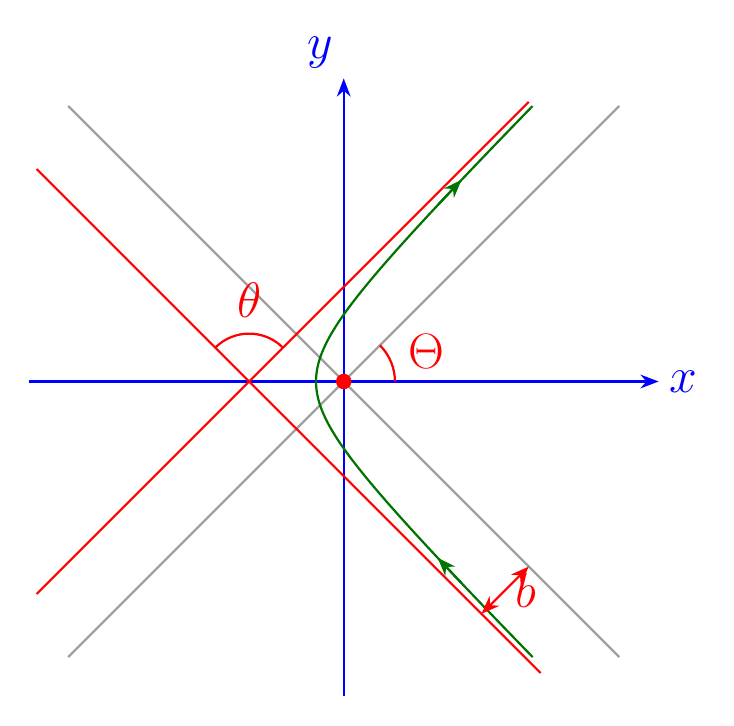
\begin{tikzpicture}[>=Stealth,thick,every node/.style={font=\fontsize{18}{22}\selectfont}]
  \draw[blue,->] (-4,0) -- (4,0) node[right] {$x$};
  \draw[blue,->] (0,-4) -- (0,3.85) node[above left] {$y$};
  \draw[gray!75] (-3.5,-3.5) -- (3.5,3.5);
  \draw[gray!75] (-3.5,3.5) -- (3.5,-3.5);
  % a=b=.85, c=.85 sqrt(2). The right focus is the force centre O.
  \pgfmathsetmacro{\c}{.85*sqrt(2)}
  \draw[red] (-3.9,{-3.9+\c}) -- (2.35,{2.35+\c});
  \draw[red] (-3.9,{3.9-\c}) -- (2.5,{-2.5-\c});
  \draw[green!45!black,
    domain=-3.5:3.5,samples=180,smooth,variable=\t]
    plot ({-\c+sqrt(.85*.85+\t*\t)},\t);
  \foreach \y in {-2.4,2.4} {
    \draw[green!45!black,->,domain={\y-.16}:{\y+.16},samples=8,variable=\t]
      plot ({-\c+sqrt(.85*.85+\t*\t)},\t);
  }
  \fill[red] (0,0) circle (2.8pt);
  \draw[red] (.65,0) arc[start angle=0,end angle=45,radius=.65];
  \node[red] at (1.05,.38) {$\Theta$};
  \draw[red] ({-\c+.43},.43) arc[start angle=45,end angle=135,radius={.43*sqrt(2)}];
  \node[red] at (-\c,1.03) {$\theta$};
  % Perpendicular distance from the incoming asymptote to its parallel through O.
  \draw[red,<->] (2.35,-2.35) -- ({2.35-\c/2},{-2.35-\c/2})
    node[midway,right] {$b$};
\end{tikzpicture}
\end{document}
